\definecolor{cfwone}{HTML}{eef5fa}
\definecolor{cfwtwo}{HTML}{daeaf5}
\definecolor{cfwthree}{HTML}{b2d2e9}
\definecolor{cfwfour}{HTML}{8abbde}

\newcommand{\fwone}[1]{\colbox{cfwone}{#1}\xspace}
\newcommand{\fwtwo}[1]{\colbox{cfwtwo}{#1}\xspace}
\newcommand{\fwthree}[1]{\colbox{cfwthree}{#1}\xspace}
\newcommand{\fwfour}[1]{\colbox{cfwfour}{#1}\xspace}

\newcommand{\fexp}[2]{\texttt{[{\color{darkgray}{#1:#2}}]}\xspace}
\newcommand{\fexptag}[1]{\fexp{TAG}{#1}}
\newcommand{\fexpfrom}[1]{\fexp{FROM}{#1}}
\newcommand{\fexpto}[1]{\fexp{TO}{#1}}
\newcommand{\fexptemp}[1]{\fexp{TEMP}{#1}}


\section{\sysname for Explanations}
\label{sec:app_explain}
%Both counterfactual explanations and semi-counterfactual explanations.
%As defined in \cite{}




\begin{figure}[t]
\centering
\includegraphics[trim={0 21cm 33cm 0cm},clip,width=1\columnwidth]{figures/explanation_v2.pdf}
\vspace{-15pt}
\caption{
(A) A \qqp instance with explanations and predictions ($\mathbf{=}$ means \emph{Duplicate}, $\mathbf{\not\eq}$ \emph{Non-Duplicate}), as well as the feature weights from SHAP.
Counterfactual explanations complement SHAP, \ie they (B) concretize the opaque weights using readable examples, and (C, D) alert abnormalities missed by SHAP.
}
\vspace{-10pt}
\label{fig:explanation}
\end{figure}

Counterfactual explanations have been elusive in NLP, despite evidence from social science research~\cite{miller} indicating that they may be more intuitive than feature attribution methods. 
Compared to the opaque feature weights in Figure~\ref{fig:explanation}A, Figure~\ref{fig:explanation}B more intuitively show that the BERT \qqp model\footnote{\url{https://huggingface.co/textattack/bert-base-uncased-QQP}} considers ``help'' trivial: 
\swap{help}{find} in \emph{Q2} does not change the prediction.

%

Here, we first select counterfactuals to serve as local explanations in \S\ref{subsec:local_explain}, and evaluate their effectiveness in \S\ref{subsec:exp_user_study}.
We discuss the use of $\xp$ beyond local explanations in \S\ref{subsec:exp_more}.

%\wts{Finding bugs missed by the feature attribution, and concretizing the opaque weights using readable examples.}
\subsection{Selection: Abnormalities as Explanations}
\label{subsec:local_explain}


Because complete explanations is overwhelming, \citet{miller} concluded that people usually only expect explanations on contrastive cases (``foils'') that they consider \emph{abnormal}.
We similarly select abnormal counterfactuals as explanations, \ie counterfactuals where \emph{the expected and the actual changes in the prediction do not match}.
In other words, the relationship $\relation{\xp}$ used in the selection is \emph{the change of model prediction.}

Given a model $f$, we define the actual prediction change as $\dist(\fp, x)=|\fp(\xp)-\fp(x)|$, where $\fp(x)$ denotes the prediction probability of $f$ on $x$.
Meanwhile, the \emph{human expectation} on the prediction change is $\E[\dist(\xp, x)]$.
The mismatch between the expectation and reality is then:
$$\Delta\dist(\xp, x) = \dist(\xp, x)-\E[\dist(\xp, x)]$$
We select two \emph{expectation violation} counterfactuals, \ie (1) large prediction change from trivial perturbations (small expectations): $\xp_L = \argmax_{\xp} \Delta\dist(\xp, x)$, or (2) unchanged predictions from large changes: $\xp_U = \argmax_{\xp} -\Delta\dist(\xp, x)$. 

%  (\eg for measuring ), model-agnostic~\cite{reimers-2019-sentence-bert} or dependent on the hidden layer of the model. The embedding can be either model-agnostic~\cite{reimers-2019-sentence-bert}, or the hidden state of a finetuned predictor

$\E[\boldsymbol{\cdot}]$ can take various forms.
Though we can use the cosine distance in the latent space~\cite{reimers-2019-sentence-bert} to select standalone explanations, a more effective use case is to \emph{complement} existing feature attribution methods.
%, which are not available in pure counterfactual explanations. However, as mentioned in \S\ref{sec:relate}, they only
Methods like SHAP~\cite{NIPS2017_7062} or LIME~\cite{Ribeiro2016WhySI} provide overviews of features weights, which are not available in pure counterfactual explanations.
However, they estimate weights by \emph{masking} words, and therefore cannot reflect how models would react to replacements or additions.

To highlight this usually overlooked nuance, we define $\E[\boldsymbol{\cdot}]$ using the importance (weights) of the perturbed tokens in $x$, estimated by SHAP.
Abnormalities selected this way highlight the missed pieces, and better calibrate users' trust in the predictor. 
Figure~\ref{fig:explanation}C shows such a $\xp_L$: \swap{friend}{woman} changes the prediction from \emph{Duplicate} to \emph{Non-Duplicate}, even though ``friend'' is trivial according to SHAP; Whereas changing the important ``in depression'' in Figure~\ref{fig:explanation}D still results in \emph{Duplicate} ($\xp_U$).
Detailed distance functions are in \S\ref{appendix:exp_rank}.



\subsection{Evaluation on Local Explanations}
\label{subsec:exp_user_study}

We conduct a user study to verify whether our local counterfactual explanations can complement SHAP.
%, as the setup nicely combines the overview provided by SHAP, and the decision boundaries it omits.
%\footnote{We defer more sophisticated designs and evaluations for interactive and global explanation to future work.}
%, where participants are asked to predict model's behavior on the given variations of a base example.
The study takes the form of counterfactual simulation~\cite{hase2020evaluating}, with participants predicting a model's behavior on counterfactuals.
Intuitively, the more they simulate incorrectly, the more information they grasp \emph{if we show the counterfactuals to them}.

\paragraph{Procedure.}
We recruited 13 graduate students who have intermediate NLP knowledge and have experience using model explanations, and asked them to simulate the aforementioned \qqp model for 20 rounds.
In each round, the participants were given a base example with the model's prediction, as well as the SHAP weights, highlighted in the text and with a bar chart (Figure~\ref{fig:explanation}A).
Moreover, they could create up to ten counterfactuals on their own, and query the model predictions on them.
More interactions with the predictor usually result in better mental models~\cite{miller}, and we are interested in whether our selected ones \emph{still add information} after such nearly unlimited model access (participants submitted $6.3\pm3.2$ queries per round.)
Participants then simulated the model's predictions on six given counterfactuals, two from each of the following three conditions.
We concluded the study with open-ended questions on their counterfactual creation and simulation strategies.

%We validate this hypothesis in user study, where expert users did slightly better than random (accuracy: $55 \pm 6\%$) at predicting what a model would do on \sysname counterfactuals, even after seeing SHAP explanations \cite{NIPS2017_7062} and manually creating counterfactuals to explore the model's behavior. This indicates that seeing such explanations would add a lot of information that users are currently missing (much of which consisting of mistaken model predictions) even if when they perform manual counterfactual analysis and use feature attribution methods.


\newcommand{\cshap}{\emph{SHAP-c}\xspace}
\newcommand{\crandom}{\emph{Random}\xspace}
\newcommand{\chuman}{\emph{Human}\xspace}
\paragraph{Conditions.} 
We compare three types of counterfactuals:
(1) \cshap, the \sysname-generated counterfactuals, selected to complement SHAP; 
(2) \crandom, the randomly selected \sysname counterfactuals; 
(3) \chuman, the human generated counterfactuals, in which two graduate students (that were not in the actual study) played with the model, and each created one $\xp$ where the model prediction was incorrect and counterintuitive according to the SHAP score on the base example.

\begin{comment}
\begin{figure}[t]
\centering
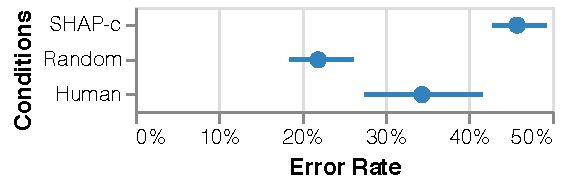
\includegraphics[width=1\columnwidth]{figures/err_rate.pdf}
\vspace{-15pt}
\caption{
Error rates on counterfactuals in different conditions. The higher the error rate, the more information missed by the participants, therefore can better complement manual counterfactual analysis and SHAP.
}
\vspace{-10pt}
\label{fig:err_rate}
\end{figure}
\end{comment}

\paragraph{Results.}
As a within-subject study, we compared \emph{the error rate of human simulations across the three conditions}.
%As in Figure~\ref{fig:err_rate}, 
Participants were able to simulate the cases in \crandom (error rate $e=23\%\pm6\%$), possibly because \crandom selections contained more minor variations that aligned with the SHAP values and participants' intuitions.
They missed more \chuman ($e=39\%\pm11\%$) cases, and were even slightly worse on \cshap ($45\%\pm 6\%$, only slightly better than random guess).%, though the confidence intervals overlap.

This shows that \cshap counterfactuals were beyond participants' learnings from feature attributions and manual counterfactual analysis, and \emph{would still add value if they were presented.}
They were also at least as effective as the \chuman condition, which is very expensive to create --- each graduate student spent 1.5-2 hours on the task.


Usually, participants simulated the model incorrectly because they missed the inspection spots.
For example, they repeatedly perturbed ``depression'' in Figure~\ref{fig:explanation}A, and therefore had to ``guess using intuitions'' when simulating Figure~\ref{fig:explanation}B.
However, in 24\% of the missed \cshap cases, participants successfully covered the related pattern,\footnote{At least one of their queries perturbed the same spans as the given counterfactual, and the text overlap between the query and the counterfactual was over 70\%.} but were misled by their inspections --- ``labeled based on similar examples I tried,'' as one subject articulated.
It was hard for them to imagine model predicting \emph{Duplicate} on Figure~\ref{fig:explanation}B (\swap{help}{find}), when the model predicted \emph{Non-Duplicate} on their query \exinline{How do I \swap{help}{play with}...?}
The number dropped to $15\%$ for the \chuman condition.
In other words, \emph{\cshap found more bugs within spots where humans considered inspected.}
%\hao{this is very interesting. close by summarizing the conclusion?}

\noindent\textbf{Takeaway.}
\sysname counterfactuals complement feature attribution methods and counterfactual analysis, as effectively as hiring a second expert for the analysis (but much cheaper).
In particular, they highlight erroneous spots where humans may be misled by their own analysis.

\subsection{Beyond Local Explanations}
\label{subsec:exp_more}

\paragraph{Interactive explanations: user-selected abnormalities.}
%\paragraph{Interactive explanation.}
Automated selections focus on general abnormality, but users should be able to point towards the part \emph{they} do not understand~\cite{miller}.
%Furthermore, the method should allow explanations as a dialog. 
The targeted generation seamlessly supports such interactive explanation.
For example, an analyst can follow up on Figure~\ref{fig:explanation}C by \texttt{BLANK}ing ``friend'' in Q2, and observe the model's unstable behaviors: it predicts \emph{Non-duplicate} when \remove{friend} is changed to \add{woman}, \add{kid}, \add{professional}, but remains \emph{Duplicate} when the noun is \add{man}, \add{student}.


\paragraph{Global Explanations: Recurring edits with unclear impact.}
\label{subsec:global_exp}
%\paragraph{Global explanations: impacts of same changes.}
\emph{Global} explanations provide systematic understandings beyond individual instances --- yet another important aspect of model understanding~\cite{miller}.
We define global abnormality as \emph{perturbation patterns whose impacts on the prediction are hard to generalize}.
To locate them, we group counterfactuals based on their $\relation{\xp}$, which includes 
\{\ tokens removed from $x$, added to $\xp$, and the corresponding \tagstr.\ \}
Then, we select groups that contain counterfactuals with unstable prediction changes, quantified as large entropy on $(f(x) \veryshortarrow f(\xp))$.
For example, when evaluating the \nli RoBERTa model in \S\ref{subsec:contrast_set}, one global abnormality is \swap{two}{three} in the hypothesis.
Out of the 253 $\xp$ whose original $f(x)=$ \emph{entailment}, $138$ flipped to \emph{contradiction}, $22$ to \emph{neutral}, yet $93$ remained \emph{entailment}, resulting in entropy $I=0.91$.
We observe that most cases flipped to \emph{contradiction} have the explicit word ``two'' in the premise, whereas the prediction-intact ones suggest that the model struggles with counting:

\ebox{
\textbf{P}: Two women having drinks at the bar.\\
\textbf{H}: \swap{Two}{Three} women are at a bar.\\
\textbf{$\mathbf{f(x)\rightarrow f(\xp)}$}: \swap{entailment}{contradiction}\\
--\\
\textbf{P}: A boy and a girl gaze in a clothing store window.\\
\textbf{H}: \swap{Two}{Three} kids are looking in a store window.\\
\textbf{$\mathbf{f(x)\rightarrow f(\xp)}$}: \swap{entailment}{entailment}
}

